\section{实例验证}
\subsection{实验环境}
本实验采用10核、2.50 GHz处理器、内存为64GB的计算机、显卡为 NVIDIA GeForce RTX3090,基于Python 3.9.18的编程环境。实验中,使用pyautocad连接AutoCAD,同时读取图纸信息,最终将算法获取到的图纸信息,利用pyautocad重新写回AucoCAD中进行可视化分析,同时便于后续设计者修改。
\subsection{超参数设置}
在实验中,算法用到的模型超参数设置如下:
\begin{table}[!htb]
    \caption{\label{tab:hyper_para}超参数设置}
    \centering
    \linespread{1.25}\selectfont
    % 调整表格缩放
    \begin{tabular}{cccc}
        \hline
        模块                    & 参数名               & 数值    & 作用   \\
        \hline
        \multirow{4}{*}{D3QN} & $\alpha$          & 0.001 & 调整模型学习速度 \\
                              & $batch\_size$     & 64    & 训练数量样本 \\
                              & $\tau$            & 0.005 & 调整网络更新速度 \\
                              & $\gamma$          & 0.99  & 折扣因子 \\
        \hline
        \multirow{5}{*}{PER}  & $memory\_size$    & 2000  & 经验池大小 \\
                              & $\epsilon$        & 0.01  & 扰动因子 \\
                              & $\alpha$          & 0.6   & 调整优先级的重要性 \\
                              & $abs\_err\_upper$ & 1     & 误差裁剪上限 \\
                              & $\Delta \beta$    & 0.01  & 重要性采样调整速度 \\
        \hline
    \end{tabular}
\end{table}

\subsection{地库自动化排布实验}
\subsubsection{图纸参数}
本实验共使用了6张不同属性的CAD工程图纸进行对比实验,这些图纸的属性均有不同之处,其中图纸2、4为大规模、多边界点、多障碍图纸,1、5为高密度小图纸(障碍在图纸中占比较大且图纸总面积小)。具体信息如表~\ref{tab:drawing_info}所示。
\begin{table}[!htb]
    \caption{\label{tab:drawing_info}图纸信息}
    \centering
    \linespread{1.5}\selectfont
    % 调整表格缩放
    \begin{tabular}{cccc}
        \hline
        编号 & 总面积 & 外边界顶点数 & 障碍群个数\\ 
        \hline
        1  & 23175  & 12 & 6   \\
        2  & 36928  & 91 & 14  \\
        3  & 23175  & 12 & 3   \\
        4  & 75388  & 24 & 22  \\
        5  & 22728  & 6  & 9   \\
        6  & 24869  & 10 & 8   \\
        \hline
    \end{tabular}
\end{table}
\subsubsection{实验结果与分析}
为了验证算法的可行性和有效性,需对每张图纸按照确定参数进行车位排布。同时,本文选择王潇霆\cite{1022674189.nh}提出的方法与人工排布作为算法对照组,其中王采用的是基于强化学习思想的探索策略和区域分割,与本文的PER-D3QN在思想上同属强化学习算法,具有一定的时间和正确性参考,同时,与平常使用的人工排列进行比较,更符合实际。根据实际情况,本文设定车位长为6m、宽为2.5m,道路宽为6m,柱子宽为0.5m。根据这些信息可进行下一步的车位布局,最终结果如表~\ref{tab:paving_situation} 所示。
\begin{table}[!htb]
    \caption{\label{tab:paving_situation}图纸排列情况}
    \centering
    \linespread{1.5}\selectfont
    % 调整表格缩放
    \begin{tabular}{ccccc}
        \hline
        \multirow{2}{*}{编号} & \multicolumn{3}{c}{车位总数} & \multirow{2}{*}{时间/min} \\ 
        \cline{2-4}
         & 王 & 人工 & 本文 & \\ 
        \hline
        1  & 621  & 605  & 576  & 18  \\
        2  & 838  & 813  & 875  & 45  \\
        3  & 725  & 630  & 752  & 19  \\
        4  & -    & 1120 & 1474 & 84 \\
        5  & 546  & 510  & 491  & 17  \\
        6  & 684  & 651  & 692  & 20  \\
        \hline
    \end{tabular}
\end{table}

针对图纸结果分析可得:
\begin{enumerate}
    \item 本文的算法在处理大规模和复杂障碍的图纸时表现出了优势。这是因为算法能够有效地处理复杂的环境,并在有限的空间内最大化车位的数量。
    \item 虽然出入口的引入导致空地空间进一步减少,但在排布中,并未产生较大影响,仍能充分利用剩余空间。
    \item 在障碍和边界上的车位铺设更具灵活性。这是因为算法能够根据环境的变化动态地调整车位的布局。
    \item 智能体既能根据获取周边状态矩阵的信息,又可以获取距离周边全局考虑车位的布局,使得车位的布局更加合理。这说明算法能够考虑全局和局部的信息,从而得到更优的布局。
    \item 但对于高密度小型图纸,由于奖励设置中只考虑了直路带来的奖励,而未考虑到转向时的奖励,因此本文算法有一定的局限性,无法获得更好的奖励。
\end{enumerate}

下面为其中几张图纸排布结果的效果展示:

\begin{figure}[!htb]
    \centering
    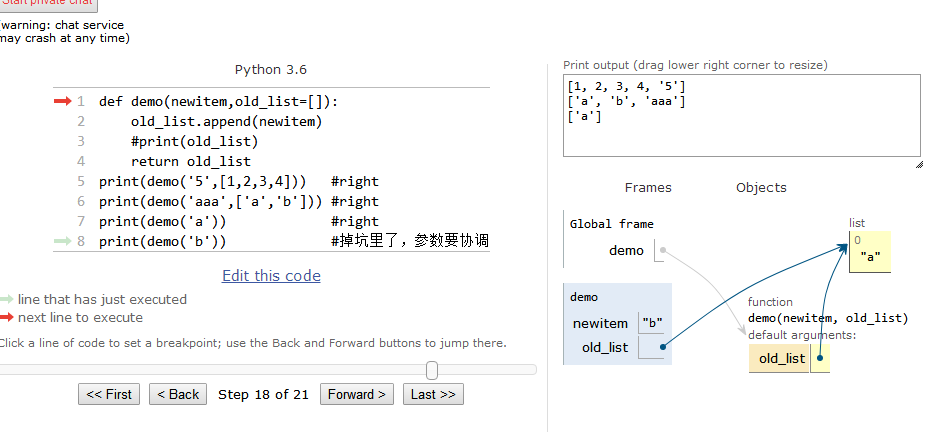
\includegraphics[width=\textwidth]{5/2}
    \caption{2号图纸排布效果}
\end{figure}

\begin{figure}[!htb]
    \centering
    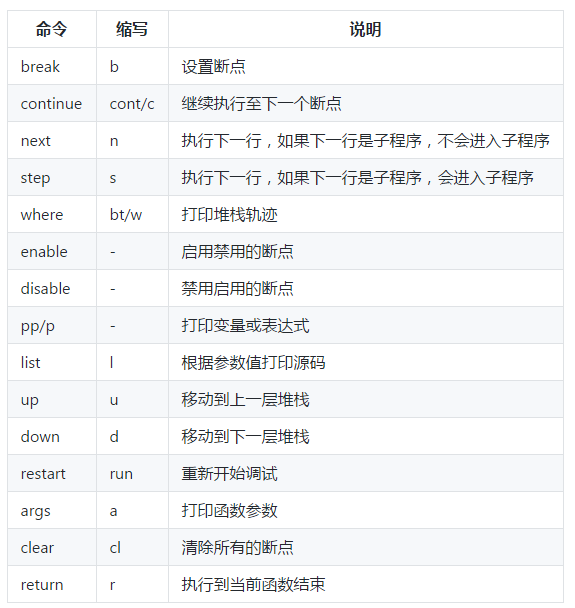
\includegraphics[width=\textwidth]{5/3}
    \caption{3号图纸排布效果}
\end{figure}
\begin{figure}[!htb]
    \centering
    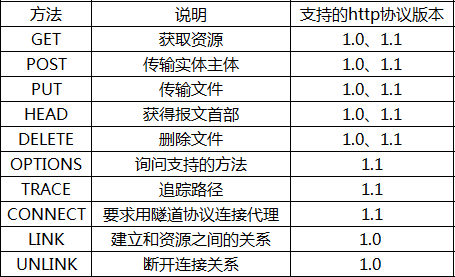
\includegraphics[width=\textwidth]{5/4}
    \caption{4号图纸排布效果}
\end{figure}

\begin{figure}[!htb]
    \centering
    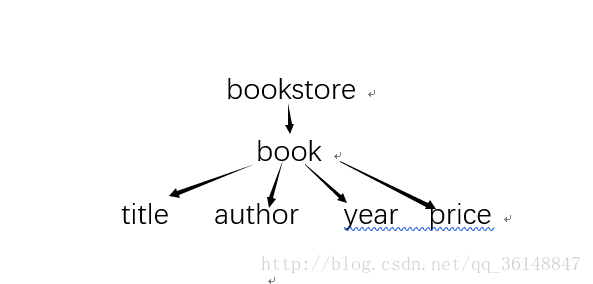
\includegraphics[width=\textwidth]{5/6}
    \caption{6号图纸排布效果}
\end{figure}